
\par\noindent\textit{命题~\ref{prop:7-2-211} 的证明。}
仍按上文定义的序关系，在 $(\ell,i)$ 上作双重归纳，
把 $\widehat{\mathfrak C}'_i$ 与 $\mathcal I'_i$
分别提升为滤过
$A_{\bar n(\lambda_{i+\ell}),\bar k(\lambda_{i+\ell})}$
代数与同态。$\ell=0$ 时无需证明。
假定所有 $(\ell',i')<(\ell,i)$ 的情形均已构造，
现考虑 $(\ell,i)$。记
$(\bar n(\lambda_{i+\ell}),\bar k(\lambda_{i+\ell}))=(n',K')$。
由于 $(\ell-1,i+1)<(\ell,i)$，
归纳假设给出 $\widehat{\mathfrak C}'_{i+1}$
上的滤过 $A_{n',K'}$ 结构及映射 $\mathcal I'_{i+1}$。
设 $\widehat{\mathfrak C}'_i$ 与 $\mathcal I'_i$
的滤过 $A_{n,K}$ 结构已给定；
可假定 $((n,K),(n',K'))$ 属于
(7.2.130.1) 或 (7.2.130.2) 的类型。

由于
$\mathcal I'_i\colon
\widehat{\mathfrak C}'_{i,r=1}
\to\widehat{\mathfrak C}'_{i+1,r=0}$
是 $A_{n,K}$ 同伦等价，
由定理~\ref{thm:7-2-72}，
可以把 $\widehat{\mathfrak C}'_{i,r=1}$
及 $\mathcal I'_i$ 提升至滤过 $A_{n',K'}$
层次，使后者成为滤过 $A_{n',K'}$ 同态。
还可证明如下引理。

\begin{lemma}{7.2.225}\label{lem:7-2-225}
可以将 $\widehat{\mathfrak C}'_{i,r=1}$
上的滤过 $A_{n,K}$ 结构与 $\mathcal I'_i$
一并提升至滤过 $A_{n',K'}$ 层次，使
\[
\operatorname{Eval}_{s=s_0}\circ\mathcal I'_i
=I'_i\circ\operatorname{Eval}_{s=s_0}
\]
也在滤过 $A_{n',K'}$ 同态层次上作为等式成立。
\end{lemma}

\begin{proof}
先选取 $\mathfrak m^I_{K',\beta}$ 与
$(\mathcal I'_i)^I_{K',\beta}$，
使 $\mathfrak m^I_{K',\beta}$ 给出
$\widehat{\mathfrak C}'_{i,r=1}$ 上的滤过
$A_{n',K'}$ 结构，且 $\mathcal I'_i$
成为滤过 $A_{n',K'}$ 同态。
此时不要求
$\overline{\operatorname{Eval}}_{s=s_0}\colon
\widehat{\mathfrak C}'_{i,r=1}
\to\widehat{\mathfrak C}'_{i,r=1,s=s_0}$
是滤过 $A_{n',K'}$ 同态。
上述选取由定理~\ref{thm:7-2-72} 保证。
对 $\lVert\beta\rVert=n'$，置
\[
\begin{aligned}
\operatorname{Err1}_{K',\beta,s_0}
&=\overline{\operatorname{Eval}}_{s=s_0}
\circ\mathfrak m^I_{K',\beta}
-\mathfrak m_{K',\beta}\circ
\overline{\operatorname{Eval}}_{s=s_0}^{\otimes K'}\\
&\in\operatorname{Hom}\bigl(
B_{K'}(\overline{\widehat{\mathfrak C}}'_{i,r=1}[1]),
\overline{\widehat{\mathfrak C}}'_{i,r=1,s=s_0}[1]
\bigr).
\end{aligned}
\]
有公式
\[
\begin{aligned}
(I'_i)_{1,0}\circ\operatorname{Err1}_{K',\beta,s=s_0}
&=\sum_{\beta_1+\beta_2=\beta}
\sum_{k_1+k_2=K'+1}
\Bigl((I'_i)_{k_1,\beta_1}\circ
\overline{\operatorname{Eval}}_{s=s_0}^{\otimes k_1}
\circ\widehat{\mathfrak m}^{I}_{k_2,\beta_2}\\
&\hspace{5em}-(I'_i)_{k_1,\beta_1}\circ
\widehat{\mathfrak m}_{k_2,\beta_2}
\circ\overline{\operatorname{Eval}}_{s=s_0}^{\otimes K'}
\Bigr).
\end{aligned}
\]
上式中的 $\mathfrak m^I_{k_2,\beta_2}$，
除 $(k_2,\beta_2)=(K',\beta)$ 外，
均表示 $\widehat{\mathfrak C}'_{i,r=1}$
上已给定的滤过 $A_{n,K}$ 结构。
利用引理中的等式已在 $A_{n,K}$ 同态层次成立，
并且 $I'_i$ 是 $A_{n',K'}$ 同态，得到
\[
\begin{aligned}
(I'_i)_{1,0}\circ\operatorname{Err1}_{K',\beta,s_0}
=-\delta_1\Bigl(
(I'_i)_{K',\beta,0}\circ
\overline{\operatorname{Eval}}_{s=s_0}^{\otimes K'}
-\overline{\operatorname{Eval}}_{s=s_0}\circ
(\mathcal I'_i)^I_{K',\beta}
\Bigr).
\end{aligned}
\]
此处及以下均记
\[
\delta_1(A)=\overline{\mathfrak m}_1\circ A
-(-1)^{\deg A}A\circ\widehat{\mathfrak m}_1.
\]
此外，$\operatorname{Err1}_{K',\beta,s_0}$
是 $\delta_1$-圈。因此存在
\[
\operatorname{Cor1}_{K',\beta,s=s_0}
\in\operatorname{Hom}\bigl(
B_{K'}(\overline{\widehat{\mathfrak C}}'_{i,r=1}[1]),
\overline{\widehat{\mathfrak C}}'_{i,r=1,s=s_0}[1]
\bigr)
\]
满足
\[
\operatorname{Err1}_{K',\beta,s=s_0}
=\delta_1(\operatorname{Cor1}_{K',\beta,s=s_0}).
\]
又存在
$\operatorname{Cor2}_{K',\beta}\in
\operatorname{Hom}\bigl(
B_{K'}(\overline{\widehat{\mathfrak C}}'_{i,r=1}[1]),
\overline{\widehat{\mathfrak C}}'_{i,r=1}[1]
\bigr)$，使
\[
\overline{\operatorname{Eval}}_{s=s_0}\circ
\operatorname{Cor2}_{K',\beta}
=\operatorname{Cor1}_{K',\beta,s=s_0}.
\]
置
\[
\mathfrak m^{II}_{K',\beta}
=\mathfrak m^I_{K',\beta}
-\delta_1(\operatorname{Cor2}_{K',\beta}).
\]
这使相应分量在 $\widehat{\mathfrak C}'_{i,r=1}$
上定义滤过 $A_{n',K'}$ 结构，
且 $\overline{\operatorname{Eval}}_{s=s_0}$
成为滤过 $A_{n',K'}$ 同态。
再置
\[
(\mathcal I'_i)^{II}_{K',\beta}
=(\mathcal I'_i)^I_{K',\beta}
-(\mathcal I'_i)_{1,0}\circ
\operatorname{Cor2}_{K',\beta}.
\]
它在结构 $\mathfrak m^{II}_{K',\beta}$ 下
定义滤过 $A_{n',K'}$ 同态。

接下来考虑\translatornote{原书此处把
$\mathcal I'_i$、$I'_i$ 间歇写成无撇形式，
译稿按引理所定源靶统一撇号；
$\operatorname{Err3}$、$\operatorname{Cor3}$
的 $(K,\beta_0)$ 与随后
$\operatorname{Cor4}$ 的 $(K',\beta)$
则暂保留源文混用，待核。}
\[
\begin{aligned}
\operatorname{Err3}_{K,\beta_0,s=s_0}
&=\overline{\operatorname{Eval}}_{s=s_0}\circ
(\mathcal I'_i)^{II}_{K',\beta}
-(I'_i)_{K',\beta}\circ
\overline{\operatorname{Eval}}_{s=s_0}^{K'\otimes}\\
&\in\operatorname{Hom}\bigl(
B_{K'}(\overline{\widehat{\mathfrak C}}'_{i,r=1}[1]),
\overline{\widehat{\mathfrak C}}'_{i+1,r=0,s=s_0}[1]
\bigr).
\end{aligned}
\]
它是 $\delta_1$-圈，且
\[
\begin{aligned}
\operatorname{Err3}_{K,\beta_0,s=s_0}
&-\Bigl(
\overline{\operatorname{Eval}}_{s=s_0}\circ
(\mathcal I'_i)^I_{K',\beta}
-(I'_i)_{K',\beta}\circ
\overline{\operatorname{Eval}}_{s=s_0}^{K'\otimes}
\Bigr)\\
&=-(I'_i)_{1,0}\circ
\operatorname{Cor1}_{K',\beta,s=s_0}.
\end{aligned}
\]
选取 $\operatorname{Cor1}_{K',\beta,s=s_0}$ 时，
可加上一个 $\delta_1$-圈而不改变上述条件。
利用这项自由度，可假定
$\operatorname{Err3}_{K,\beta_0,s=s_0}$
是 $\delta_1$-边界。
取如下修正项：
\[
\operatorname{Cor3}_{K,\beta_0,s=s_0}\in
\operatorname{Hom}\bigl(
B_{K'}(\overline{\widehat{\mathfrak C}}'_{i,r=1}[1]),
\overline{\widehat{\mathfrak C}}'_{i+1,r=0,s=s_0}[1]
\bigr).
\]
它满足
\[
\operatorname{Err3}_{K,\beta_0,s=s_0}
=\delta_1(\operatorname{Cor3}_{K,\beta_0,s=s_0}).
\]
再取
$\operatorname{Cor4}_{K,\beta_0}\in
\operatorname{Hom}\bigl(
B_{K'}(\overline{\widehat{\mathfrak C}}'_{i,r=1}[1]),
\overline{\widehat{\mathfrak C}}'_{i+1,r=0}[1]
\bigr)$，满足
\[
\overline{\operatorname{Eval}}_{s=s_0}\circ
\operatorname{Cor4}_{K,\beta_0}
=\operatorname{Cor3}_{K,\beta_0,s=s_0},
\]
并置
\[
(\mathcal I'_i)^{III}_{K',\beta}
=(\mathcal I'_i)^{II}_{K',\beta}
-(\mathcal I'_i)_{1,0}\circ
\delta_1(\operatorname{Cor4}_{K',\beta}).
\]
此时 $\mathfrak m^{II}_{K',\beta}$ 与
$(\mathcal I'_i)^{III}_{K',\beta}$
具有所要求的性质。
\end{proof}

取 $\beta\in\mathfrak G$、$\lVert\beta\rVert=n'$，
考虑把 $\widehat{\mathfrak C}'_i$
延拓为滤过 $A_{n',K'}$ 代数的障碍类
\[
o_{K',\beta}(\widehat{\mathfrak C}'_i)
\in\operatorname{Hom}\bigl(
B_{K'}\overline{\widehat{\mathfrak C}}'_i[1],
\overline{\widehat{\mathfrak C}}'_i[1]
\bigr).
\]
其定义见 (7.2.201)。依归纳假设计算，
\[
\begin{aligned}
\overline{\operatorname{Eval}}_{r=1}\circ
o_{K',\beta}(\widehat{\mathfrak C}'_i)
&=\sum\overline{\operatorname{Eval}}_{r=1}\circ
\widehat{\mathfrak m}_{k_1,\beta_1}
\circ\widehat{\mathfrak m}_{k_2,\beta_2}\\
&=\sum\mathfrak m_{k_1,\beta_1}\circ
\overline{\operatorname{Eval}}_{r=1}\circ
\widehat{\mathfrak m}_{k_2,\beta_2}\\
&=\sum\mathfrak m_{k_1,\beta_1}\circ
\widehat{\mathfrak m}_{k_2,\beta_2}\circ
\widehat{\overline{\operatorname{Eval}}}_{r=1}.
\end{aligned}
\]
求和遍历 $k_1,k_2,\beta_1,\beta_2$，
满足 $k_1+k_2=K'+1$、
$\beta_1+\beta_2=\beta$，且
$(k_i,\beta_i)\ne(1,\beta_0)$。
由 $A_{n',K'}$ 关系得到
\begin{equation}
\overline{\operatorname{Eval}}_{r=1}\circ
o_{K',\beta}(\widehat{\mathfrak C}'_i)
+\delta_1\bigl(
\mathfrak m_{K',\beta}\circ
\widehat{\overline{\operatorname{Eval}}}_{r=1}
\bigr)=0.
\tag{7.2.226.1}\label{eq:7-2-226-1}
\end{equation}
同理，
\begin{equation}
\overline{\operatorname{Eval}}_{s=s_0}\circ
o_{K',\beta}(\widehat{\mathfrak C}'_i)
+\delta_1\bigl(
\mathfrak m_{K',\beta}\circ
\widehat{\overline{\operatorname{Eval}}}_{s=s_0}
\bigr)=0.
\tag{7.2.226.2}\label{eq:7-2-226-2}
\end{equation}

取 $\overline C'_i$ 的两个副本
$\overline C'_{i,s=s_0,r=r_0}$，
其中 $s_0=0,1$、$r_0=1$；
参见 (7.2.189.5)\translatornote{原书此处误引
“(30.189.5)”；同段下一句正确引 (7.2.189.5)。}。
置
\begin{equation}
\mathfrak K=\ker\left(
\overline{\widehat{\mathfrak C}}'_{i,s=0}
\oplus\overline{\widehat{\mathfrak C}}'_{i,s=1}
\oplus\overline{\widehat{\mathfrak C}}'_{i,r=1}
\xrightarrow{\overline B}
\bigoplus_{s_0=0}^{1}\overline C'_{i,s=s_0,r=1}
\right).
\tag{7.2.227}\label{eq:7-2-227}
\end{equation}
这里 $\overline B$ 由 (7.2.189.5) 的映射 $B$ 诱导。

\begin{statement}{子引理}{7.2.228}\label{sublem:7-2-228}\itshape
映射
\begin{equation}
\bigl(
\overline{\operatorname{Eval}}_{s=0}
\oplus\overline{\operatorname{Eval}}_{s=1}
\oplus\overline{\operatorname{Eval}}_{r=1}
\bigr)\colon
\overline{\widehat{\mathfrak C}}'_i\longrightarrow\mathfrak K
\tag{7.2.229}\label{eq:7-2-229}
\end{equation}
良定义、满射，且为同伦等价。
\end{statement}

\par\medskip\noindent\begin{minipage}{\textwidth}
\centering
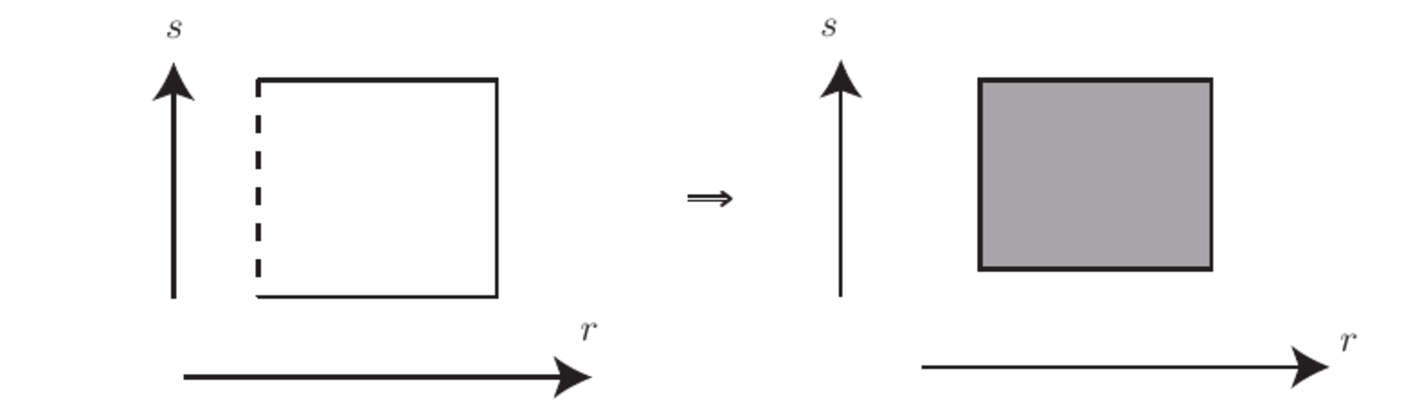
\includegraphics[width=.75\textwidth]{chapters/ch07-transversality/figures/phys-532-figure-7-2-12-crop.png}
\par{\renewcommand{\thefigure}{7.2.12}\refstepcounter{figure}
\normalfont\bfseries 图~\thefigure\label{fig:7-2-12}}
\end{minipage}\par\medskip

这是如下事实的代数对应物：
\[
\bigl(\{1\}\times[0,1]_s\bigr)
\cup\bigl([0,1]_r\times\{0,1\}\bigr)
\longrightarrow[0,1]^2
\]
是同伦等价；见图~\ref{fig:7-2-12}。

\par\noindent\textit{子引理~\ref{sublem:7-2-228} 的证明。}
良定义性显然。为证满射，取
\[
(x,y,z)\in
\overline{\widehat{\mathfrak C}}'_{i,s=0}
\oplus\overline{\widehat{\mathfrak C}}'_{i,s=1}
\oplus\overline{\widehat{\mathfrak C}}'_{i,r=1}
\]
且 $\overline B(x,y,z)=0$。
由 (7.2.192)，可找到
$w\in\overline{\widehat{\mathfrak C}}'_{i,r=0}$，
满足
\[
\bigl(\overline{\operatorname{Eval}}_{s=0}\bigr)_1(w)
=\bigl(\overline{\operatorname{Eval}}_{r=0}\bigr)_1(x),
\quad
\bigl(\overline{\operatorname{Eval}}_{s=1}\bigr)_1(w)
=\bigl(\overline{\operatorname{Eval}}_{r=0}\bigr)_1(y).
\]
于是 $\overline B(x,y,w,z)=0$。
图式~\ref{diag:7-2-6} 的正合性给出
$u\in\overline{\widehat{\mathfrak C}}'_i$，
其像为 $(x,y,z)$；满射得证。

为证 (7.2.229) 是同伦等价，
考虑下列交换图式~\ref{diag:7-2-9}。

\par\medskip\noindent\begin{minipage}{\textwidth}
\centering
\resizebox{\textwidth}{!}{$
\begin{array}{ccccccccc}
0&\longrightarrow&\overline{\widehat{\mathfrak C}}'_i
&\longrightarrow&(\overline{\widehat{\mathfrak C}}'_i)^{\oplus3}
&\longrightarrow&(\overline{\widehat{\mathfrak C}}'_i)^{\oplus2}
&\longrightarrow&0\\[1ex]
&&\downarrow&&\downarrow&&\downarrow&&\\[-.3ex]
0&\longrightarrow&\mathfrak K
&\longrightarrow&
\overline{\widehat{\mathfrak C}}'_{i,s=0}\oplus
\overline{\widehat{\mathfrak C}}'_{i,s=1}\oplus
\overline{\widehat{\mathfrak C}}'_{i,r=1}
&\xrightarrow{\overline B}&
\displaystyle\bigoplus_{s_0=0}^{1}
\overline C'_{i,s=s_0,r=1}
&\longrightarrow&0
\end{array}$}
\par{\renewcommand{\thefigure}{7.2.9}\refstepcounter{figure}
\normalfont\bfseries 图式~\thefigure\label{diag:7-2-9}}
\end{minipage}\par\medskip

竖箭头是端点评价映射或其复合。
上行的两个映射分别由
\[
x\longmapsto(x,x,x),
\qquad(x,y,z)\longmapsto(x-z,y-z)
\]
定义。图式~\ref{diag:7-2-9} 两行均正合，
第二、第三根竖箭头为同伦等价。
于是对 $R$-约化应用五引理，
再用定理 4.2.45，
第一根竖箭头也为同伦等价。
这就是说 (7.2.229) 是同伦等价，证毕。

继续证明命题~\ref{prop:7-2-211}。
先由 (7.2.192) 的正合性，取
\[
\begin{aligned}
\mathfrak m^{(1)}_{K',\beta}\colon
&B_{K'}(\overline{\widehat{\mathfrak C}}'_{i,r=0}[1])
\longrightarrow
\overline{\widehat{\mathfrak C}}'_{i,r=0}[1],\\
\mathfrak m^I_{K',\beta}\colon
&B_{K'}(\overline{\widehat{\mathfrak C}}'_i[1])
\longrightarrow
\overline{\widehat{\mathfrak C}}'_i[1],
\end{aligned}
\]
使以下四个等式成立：
\[
\begin{aligned}
\overline{\operatorname{Eval}}_{s=s_0}\circ
\mathfrak m^{(1)}_{K',\beta}
&=\mathfrak m_{K',\beta}\circ
\overline{\operatorname{Eval}}_{s=s_0}^{\otimes K'}
&&\colon B_{K'}(\overline{\widehat{\mathfrak C}}'_{i,r=0}[1])
\to\overline{\widehat{\mathfrak C}}'_{i,r=0,s=s_0}[1],\\
\overline{\operatorname{Eval}}_{s=s_0}\circ
\mathfrak m^I_{K',\beta}
&=\mathfrak m_{K',\beta}\circ
\overline{\operatorname{Eval}}_{s=s_0}^{\otimes K'}
&&\colon B_{K'}(\overline{\widehat{\mathfrak C}}'_i[1])
\to\overline{\widehat{\mathfrak C}}'_{i,s=s_0}[1],\\
\overline{\operatorname{Eval}}_{r=1}\circ
\mathfrak m^I_{K',\beta}
&=\mathfrak m_{K',\beta}\circ
\overline{\operatorname{Eval}}_{r=1}^{\otimes K'}
&&\colon B_{K'}(\overline{\widehat{\mathfrak C}}'_i[1])
\to\overline{\widehat{\mathfrak C}}'_{i,r=1}[1],\\
\overline{\operatorname{Eval}}_{r=0}\circ
\mathfrak m^I_{K',\beta}
&=\mathfrak m^{(1)}_{K',\beta}\circ
\overline{\operatorname{Eval}}_{r=0}^{\otimes K'}
&&\colon B_{K'}(\overline{\widehat{\mathfrak C}}'_i[1])
\to\overline{\widehat{\mathfrak C}}'_{i,r=0}[1].
\end{aligned}
\]
此时不要求 $\mathfrak m^I_{K',\beta}$
与 $\mathfrak m^{(1)}_{K',\beta}$
已经定义滤过 $A_{n',K'}$ 结构。
由上述端面条件，
\[
o_{K',\beta}(\widehat{\mathfrak C}'_i)
+\delta_1(\mathfrak m^I_{K',\beta})
\in\operatorname{Hom}\bigl(
B_{K'}(\overline{\widehat{\mathfrak C}}'_i[1]),
\widehat{\mathfrak K}[1]
\bigr),
\]
其中 $\widehat{\mathfrak K}$ 是 (7.2.229)
的核；左侧是引理~\ref{lem:7-2-74}
意义下的障碍链。
这里已知 $s=s_0$ 与 $r=1$
各端面上具有滤过 $A_{n',K'}$ 结构。
因此由子引理~\ref{sublem:7-2-228}，
可取\translatornote{原书此处给
$\operatorname{Cor1}_{K',\beta}$ 的靶写作
$\widehat{\mathfrak K}$，但同一障碍圈
位于移位靶 $\widehat{\mathfrak K}[1]$；
此处依其等式补 $[1]$。}
\[
\operatorname{Cor1}_{K',\beta}
\in\operatorname{Hom}\bigl(
B_{K'}(\overline{\widehat{\mathfrak C}}'_i[1]),
\widehat{\mathfrak K}[1]
\bigr)
\]
使
\[
o_{K',\beta}(\widehat{\mathfrak C}'_i)
+\delta_1(\mathfrak m^I_{K',\beta})
=\delta_1(\operatorname{Cor1}_{K',\beta}).
\]

再定义
\[
\begin{aligned}
\mathfrak K(s)
&=\bigcap_{s_0=0,1}
\ker\bigl(
\overline{\operatorname{Eval}}_{s=s_0}\colon
\overline{\widehat{\mathfrak C}}'_i
\to\overline{\widehat{\mathfrak C}}'_{i,s=s_0}
\bigr),\\
\mathfrak K_{r=0}(s)
&=\bigcap_{s_0=0,1}
\ker\bigl(
\overline{\operatorname{Eval}}_{s=s_0}\colon
\overline{\widehat{\mathfrak C}}'_{i,r=0}
\to\overline{\widehat{\mathfrak C}}'_{i,s=s_0,r=0}
\bigr).
\end{aligned}
\]
仿照子引理~\ref{sublem:7-2-228}，
可证
$\overline{\operatorname{Eval}}_{r=0}\colon
\mathfrak K(s)\to\mathfrak K_{r=0}(s)$
是链同伦等价。又有
\[
o_{K',\beta}(\widehat{\mathfrak C}'_{i,r=0})
+\delta_1(\mathfrak m^{(1)}_{K',\beta})
\in\operatorname{Hom}\bigl(
B_{K'}(\overline{\widehat{\mathfrak C}}'_{i,r=0}[1]),
\mathfrak K_{r=0}(s)[1]
\bigr),
\]
并且
\[
\begin{aligned}
\overline{\operatorname{Eval}}_{r=0}\circ
\bigl(o_{K',\beta}(\widehat{\mathfrak C}'_i)
+\delta_1(\mathfrak m^I_{K',\beta})\bigr)
=\bigl(
o_{K',\beta}(\widehat{\mathfrak C}'_{i,r=0})
+\delta_1(\mathfrak m^{(1)}_{K',\beta})
\bigr)\circ
\overline{\operatorname{Eval}}_{r=0}^{\otimes K'}.
\end{aligned}
\]
$\widehat{\mathfrak K}\subset\mathfrak K(s)$。
因此存在\translatornote{原书这里把
$\operatorname{Cor2}_{K',\beta}$ 的定义域写成
$B_{K'}(\overline{\widehat{\mathfrak C}}'_i[1])$，
并在下式把 $r=0$ 端面的障碍误标为
$r=1$；译稿依 $\mathfrak m^{(1)}$ 的型别
与目标核统一为 $r=0$。}
\[
\operatorname{Cor2}_{K',\beta}
\in\operatorname{Hom}\bigl(
B_{K'}(\overline{\widehat{\mathfrak C}}'_{i,r=0}[1]),
\mathfrak K_{r=0}(s)[1]
\bigr)
\]
满足
\[
o_{K',\beta}(\widehat{\mathfrak C}'_{i,r=0})
+\delta_1(\mathfrak m^{(1)}_{K',\beta})
=\delta_1(\operatorname{Cor2}_{K',\beta}).
\]
于是定义两组修正分量\translatornote{原书第二式右侧再次写
$\mathfrak m^{(2)}_{K',\beta}$；
这里按先前选取的待修正分量
$\mathfrak m^{(1)}_{K',\beta}$ 排印。}：
\[
\begin{aligned}
\mathfrak m^{II}_{K',\beta}
&=\mathfrak m^I_{K',\beta}
-\operatorname{Cor1}_{K',\beta},\\
\mathfrak m^{(2)}_{K',\beta}
&=\mathfrak m^{(1)}_{K',\beta}
-\operatorname{Cor2}_{K',\beta}.
\end{aligned}
\]
它们分别在 $\widehat{\mathfrak C}'_i$
和 $\widehat{\mathfrak C}'_{i,r=0}$
上定义滤过 $A_{n',K'}$ 结构，并满足\translatornote{原书下列第一、第三个等式
附带的源靶型别把全模型与 $r=0$ 端面互换；
此处依各自 $\mathfrak m$ 的定义域排印。}
\[
\begin{aligned}
\overline{\operatorname{Eval}}_{s=s_0}\circ
\mathfrak m^{II}_{K',\beta}
&=\mathfrak m_{K',\beta}\circ
\overline{\operatorname{Eval}}_{s=s_0}^{\otimes K'}
&&\colon B_{K'}(\overline{\widehat{\mathfrak C}}'_i[1])
\to\overline{\widehat{\mathfrak C}}'_{i,s=s_0}[1],\\
\overline{\operatorname{Eval}}_{r=1}\circ
\mathfrak m^{II}_{K',\beta}
&=\mathfrak m_{K',\beta}\circ
\overline{\operatorname{Eval}}_{r=1}^{\otimes K'}
&&\colon B_{K'}(\overline{\widehat{\mathfrak C}}'_i[1])
\to\overline{\widehat{\mathfrak C}}'_{i,r=1}[1],\\
\overline{\operatorname{Eval}}_{s=s_0}\circ
\mathfrak m^{(2)}_{K',\beta}
&=\mathfrak m_{K',\beta}\circ
\overline{\operatorname{Eval}}_{s=s_0}^{\otimes K'}
&&\colon B_{K'}(\overline{\widehat{\mathfrak C}}'_{i,r=0}[1])
\to\overline{\widehat{\mathfrak C}}'_{i,r=0,s=s_0}[1].
\end{aligned}
\]

最后再修正，使二者与
$\overline{\operatorname{Eval}}_{r=0}$ 相容。
考虑
\[
\begin{aligned}
\operatorname{Err}_{K',\beta}
&=\overline{\operatorname{Eval}}_{r=0}\circ
\mathfrak m^{II}_{K',\beta}
-\mathfrak m^{(2)}_{K',\beta}\circ
\overline{\operatorname{Eval}}_{r=0}^{\otimes K'}\\
&\in\operatorname{Hom}\bigl(
B_{K'}(\overline{\widehat{\mathfrak C}}'_i[1]),
\overline{\widehat{\mathfrak C}}'_{i,r=0}[1]
\bigr).
\end{aligned}
\]
$\mathfrak m^{II}_{K',\beta}$ 与
$\mathfrak m^{(2)}_{K',\beta}$
同 $\overline{\operatorname{Eval}}_{s=s_0}$ 的相容性说明
\[
\operatorname{Err}_{K',\beta}
\in\operatorname{Hom}\bigl(
B_{K'}(\overline{\widehat{\mathfrak C}}'_i[1]),
\mathfrak K_{r=0}(s)[1]
\bigr).
\]
它也是 $\delta_1$-圈。
选取 $\operatorname{Cor2}_{K',\beta}$ 时，
可在上述 $r=0$ 端面的 Hom 空间中
加上一个 $\delta_1$-圈而不改变前述条件。
故可假定存在如下修正项：
\[
\operatorname{Cor3}_{K',\beta}\in
\operatorname{Hom}\bigl(
B_{K'}(\overline{\widehat{\mathfrak C}}'_i[1]),
\mathfrak K_{r=0}(s)[1]
\bigr).
\]
它满足
\[
\operatorname{Err}_{K',\beta}
=\delta_1(\operatorname{Cor3}_{K',\beta}).
\]
由 (7.2.192) 的正合性，
存在
$\operatorname{Cor4}_{K',\beta}\in
\operatorname{Hom}\bigl(
B_{K'}(\overline{\widehat{\mathfrak C}}'_i[1]),
\overline{\widehat{\mathfrak C}}'_i[1]
\bigr)$，满足
\[
\begin{aligned}
\overline{\operatorname{Eval}}_{s=s_0}\circ
\operatorname{Cor4}_{K',\beta}&=0,\\
\overline{\operatorname{Eval}}_{r=1}\circ
\operatorname{Cor4}_{K',\beta}&=0,\\
\overline{\operatorname{Eval}}_{r=0}\circ
\operatorname{Cor4}_{K',\beta}
&=\operatorname{Cor3}_{K',\beta}.
\end{aligned}
\]
最终令
$\mathfrak m^{III}_{K',\beta}
=\mathfrak m^{II}_{K',\beta}
-\delta_1(\operatorname{Cor4}_{K',\beta})$。
此时 $\mathfrak m^{III}_{K',\beta}$ 与
$\mathfrak m^{(2)}_{K',\beta}$
具有所要求的性质，
命题~\ref{prop:7-2-211} 得证。
